\section{Præsentation af data}
\label{TestAfSkalaPraesentationAfData}
%
I følgende afsnit vil det indsamlede data blive præsenteret. Dette dækker over den gennemsnitlige besvarelse til hver af de 23 skalaer, kønsfordeling i forhold til den gennemsnitlige besvarelse, fordelingen af alder og højde samt hvor glade testpersonerne er for teknologi. 
%
\begin{figure}[H]
\centering
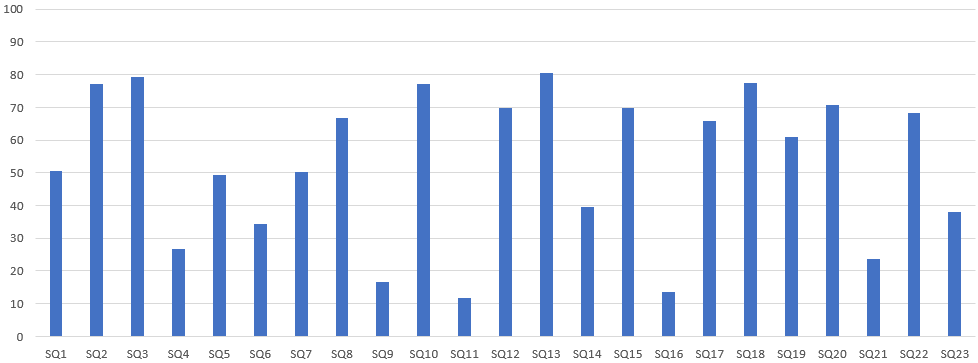
\includegraphics[width = \textwidth]{Figure/DatabehandlingSkalaer/BarPlotRaaData} 
\caption{Søjlediagram over den gennemsnitlige besvarelse til hvert skala spørgsmål.}
\label{fig:BarPlotGennemsnit}
\end{figure}
\noindent
%
På \autoref{fig:BarPlotGennemsnit} fremgår den gennemsnitlige besvarelse for hver af de 23 skalaer, angivet med \textit{Q} efterfulgt af nummer.
%
\begin{figure}[H]
\centering
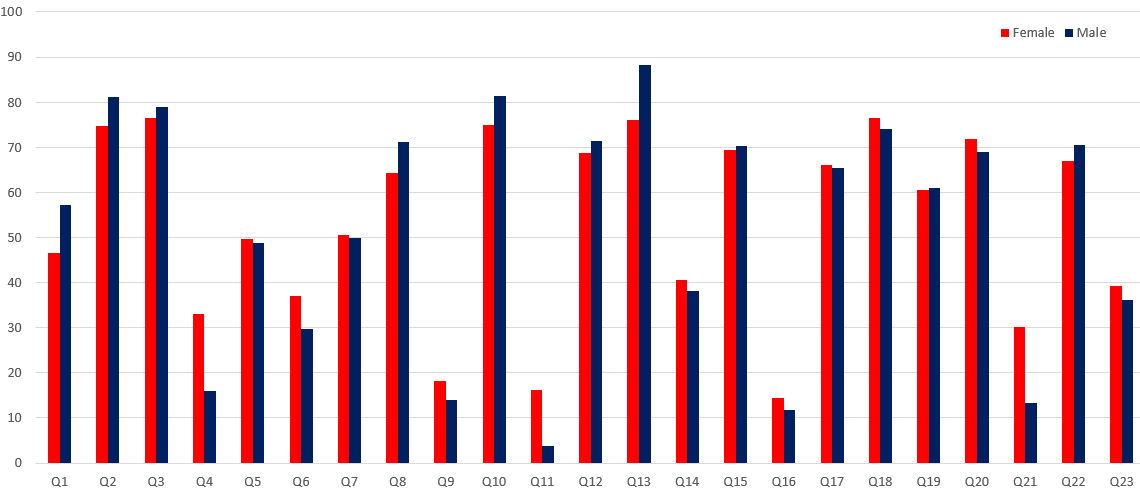
\includegraphics[width = \textwidth]{Figure/DatabehandlingSkalaer/KoenGennemnitligBesvarelser} 
\caption{Søjlediagram over den gennemsnitlige besvarelse til hvert skala spørgsmål fordelt på kvinder (rød) og mænd (blå).}
\label{fig:BarPlotKoen}
\end{figure}
\noindent
%
Baseret på \fullref{InteraktionSocialeRobotter} fremgår det, at der er kønsafhængige forskelle mellem hvordan interaktionen med sociale robotter opleves, hvilket vil blive analyseret i HENVISNING TIL AFSNIT. På \autoref{fig:BarPlotKoen} fremgår den gennemsnitlige besvarelse for hver af de 23 skalaer fordelt på køn.    
%
\begin{figure}[H]
\centering
\begin{minipage}{.5\textwidth}
  \centering
  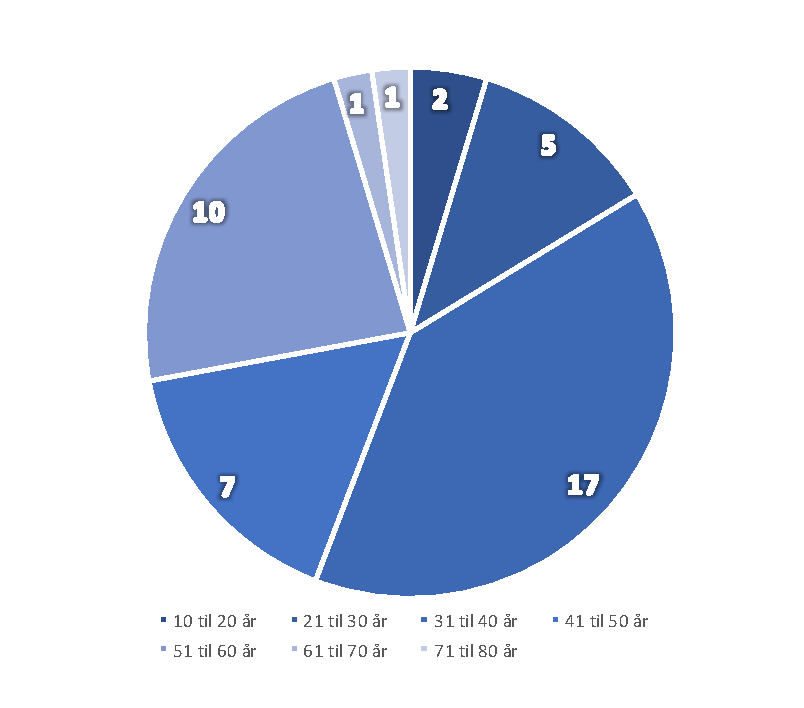
\includegraphics[width=\linewidth]{Figure/DatabehandlingSkalaer/CirkelDiagramAlder}
  \caption{Testpersonernes aldersfordeling.}
  \label{fig:CirkelDiagramAlder}
\end{minipage}%
\begin{minipage}{.5\textwidth}
  \centering
  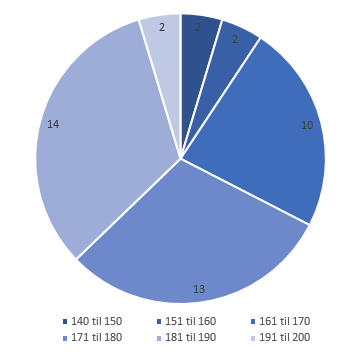
\includegraphics[width=\linewidth]{Figure/DatabehandlingSkalaer/CirkelDiagramHoejde}
  \caption{Testpersonernes højdefordeling.}
  \label{fig:CirkelDiagramHoejde}
\end{minipage}
\end{figure}
\noindent
%
Aldersfordelingen fremgår af \autoref{fig:CirkelDiagramAlder}, hvor det fremgår at størstedelen af testpersonerne har været mellem 31 år og 40 år, efterfulgt af 51 år til 60 år, med henholdvist 17 og 10 testpersoner i hver aldersgruppe. Højdefordelingen fremgår af \autoref{fig:CirkelDiagramHoejde}, hvor det fremgår at størstedelen af testpersonernes højde er mellem 161 cm til 190 cm. Mændende havde en gennemsnitshøjde på 182.1 cm (SD=6.1) og kvinderne havde en gennemsnitshøjde på 164.9 cm (SD=10.8). 
%
\begin{figure}[H]
\centering
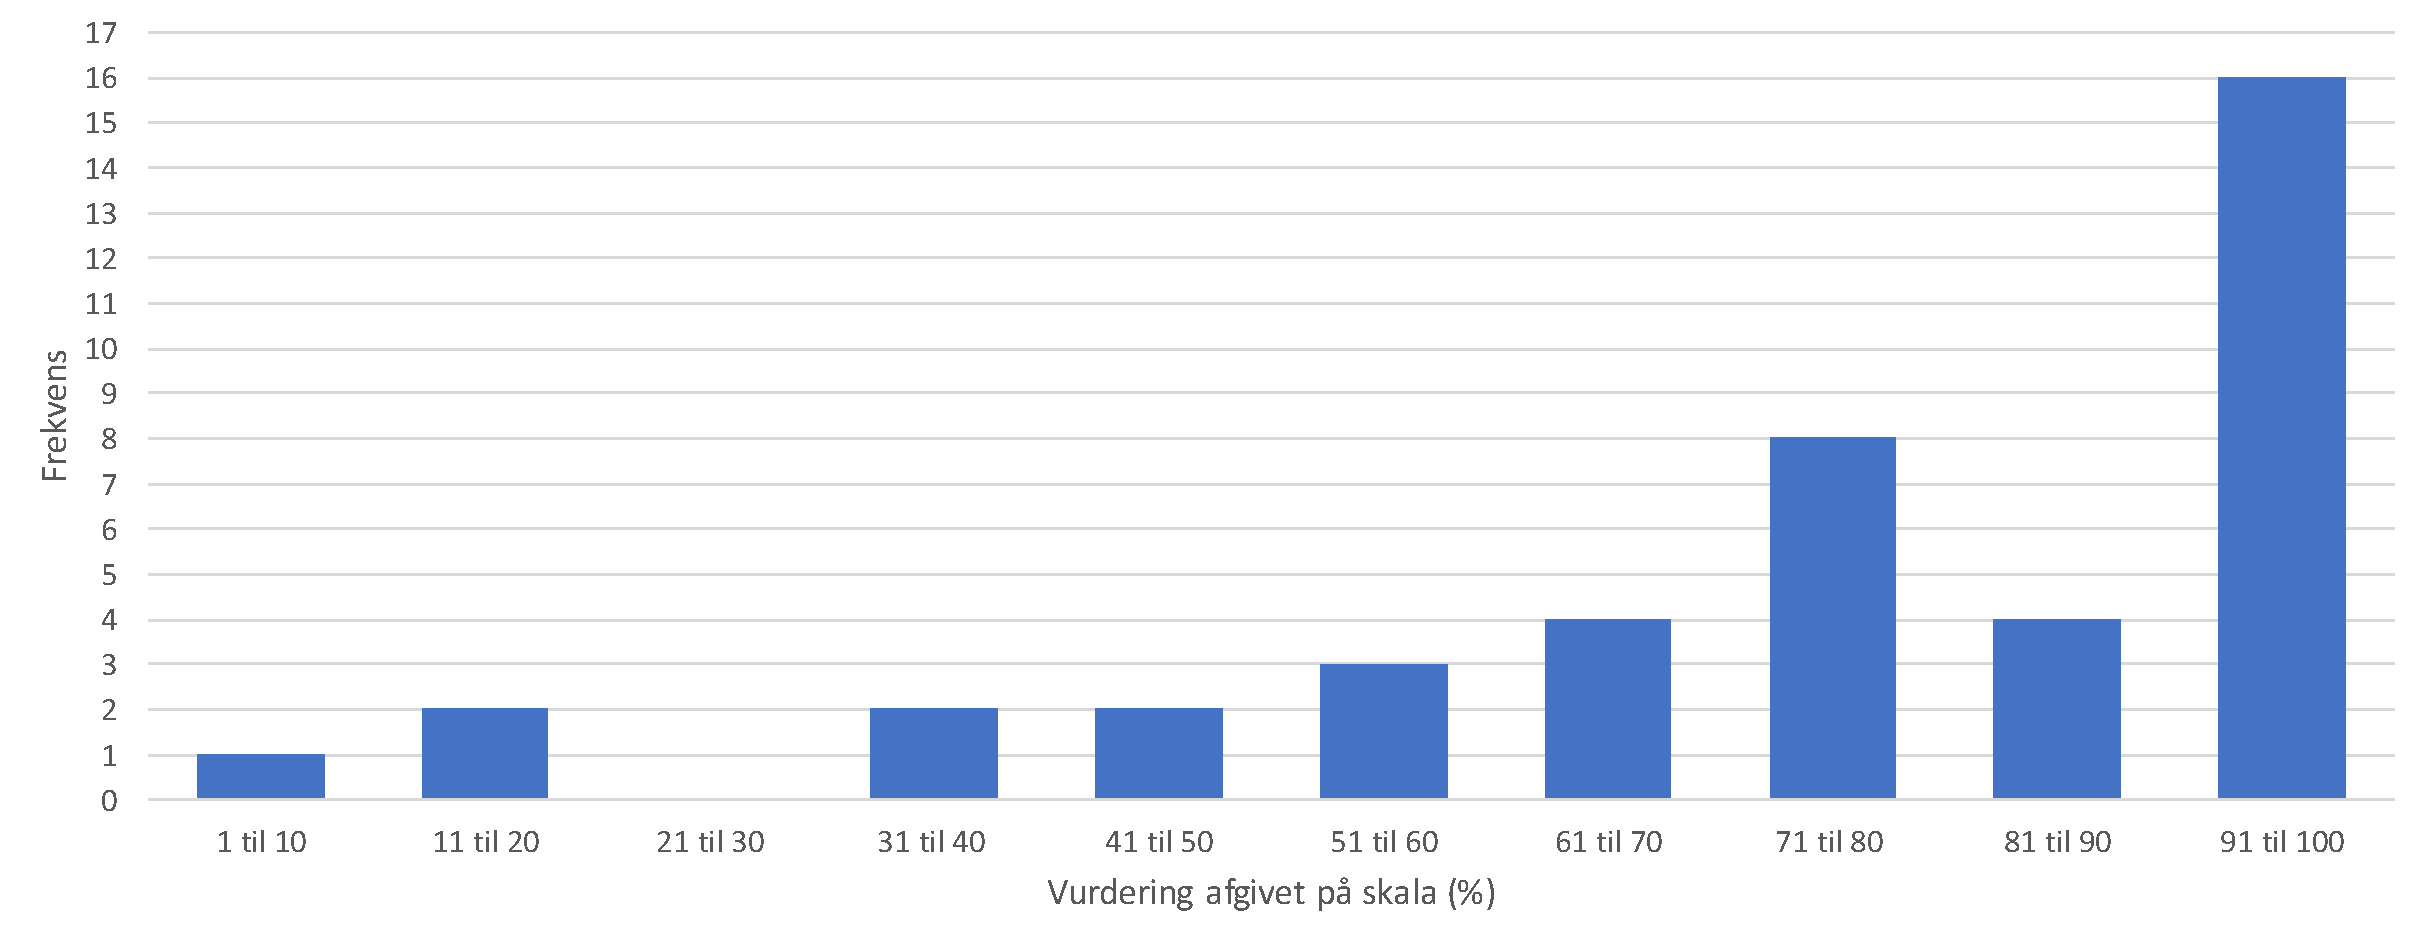
\includegraphics[width = \textwidth]{Figure/DatabehandlingSkalaer/TechFrekvens} 
\caption{Histogram over besvarelserne til skala spørgsmålet: \textit{Hvor glad er du for teknologi?}, som indgår i demografien.}
\label{fig:BarPlotTechFrekvens}
\end{figure}
\noindent
%
Baseret på \autoref{fig:BarPlotTechFrekvens} fremgår det, at størstedelen af testpersonerne er glade for teknologi, hvor 16 ud af 43 testpersoner har angivet en respons mellem 91 \% og 100 \%. Derudover tyder det på, at mændende (M=76.85, SD=22) er mere glad for teknologi end kvinderne (M=67.3, SD=30.2), fælles for begge køn er dog at standard afvigelsen er meget høj, hvorfor det ikke endeligt kan fastslåes. 
